% !TEX TS-program = pdflatex
% !TEX encoding = UTF-8 Unicode

% This is a simple template for a LaTeX document using the "article" class.
% See "book", "report", "letter" for other types of document.

\documentclass[11pt]{scrartcl} % use larger type; default would be 10pt

\usepackage[utf8]{inputenc} % set input encoding (not needed with XeLaTeX)

%%% Examples of Article customizations
% These packages are optional, depending whether you want the features they provide.
% See the LaTeX Companion or other references for full information.

%%% PAGE DIMENSIONS
\usepackage{geometry} % to change the page dimensions
\geometry{a4paper} % or letterpaper (US) or a5paper or....
% \geometry{margin=2in} % for example, change the margins to 2 inches all round
% \geometry{landscape} % set up the page for landscape
%   read geometry.pdf for detailed page layout information

\usepackage{graphicx} % support the \includegraphics command and options

% \usepackage[parfill]{parskip} % Activate to begin paragraphs with an empty line rather than an indent

%%% PACKAGES
\usepackage{booktabs} % for much better looking tables
\usepackage{array} % for better arrays (eg matrices) in maths
\usepackage{paralist} % very flexible & customisable lists (eg. enumerate/itemize, etc.)
\usepackage{verbatim} % adds environment for commenting out blocks of text & for better verbatim
\usepackage{subfig} % make it possible to include more than one captioned figure/table in a single float
\usepackage{float}
\usepackage{listings}
\usepackage{amssymb}


% These packages are all incorporated in the memoir class to one degree or another...

%%% HEADERS & FOOTERS
\usepackage{fancyhdr} % This should be set AFTER setting up the page geometry
\pagestyle{fancy} % options: empty , plain , fancy
\renewcommand{\headrulewidth}{0pt} % customise the layout...
\lhead{}\chead{}\rhead{}\lhead{}\chead{\textit{CS27020 Assignment: Ski Lifts and Pistes : jee22}}\rhead{}
\lfoot{\textit{Aberystwyth University}}\cfoot{\thepage}\rfoot{\textit{Computer Science}}

%%% SECTION TITLE APPEARANCE
\usepackage{sectsty}
\allsectionsfont{\sffamily\mdseries\upshape} % (See the fntguide.pdf for font help)
% (This matches ConTeXt defaults)

%%% ENVIRONMENT ITEMIZE
\newenvironment{myitemize}
{ \begin{itemize}[]
    \setlength{\itemsep}{0pt}
    \setlength{\parskip}{0pt}
    \setlength{\parsep}{0pt}     }
{ \end{itemize}                  } 

%%% LISTINGS LANGUAGE
\lstset{language=SQL}

%%% ToC (table of contents) APPEARANCE
\usepackage[nottoc,notlof,notlot]{tocbibind} % Put the bibliography in the ToC
\usepackage[titles,subfigure]{tocloft} % Alter the style of the Table of Contents
\renewcommand{\cftsecfont}{\rmfamily\mdseries\upshape}
\renewcommand{\cftsecpagefont}{\rmfamily\mdseries\upshape} % No bold!

%%% END Article customizations

%%% The "real" document content comes below...

\title{Brief Article}
\author{The Author}
%\date{} % Activate to display a given date or no date (if empty),
         % otherwise the current date is printed 

\begin{document}
\newpage

\begin{center}
\textbf{\LARGE CS27020}\\[0.3cm]
\textbf{\LARGE Modelling Persistent Data}\\[0.5cm]
\textbf{\LARGE Assignment: Ski Lifts and Pistes }\\[13cm]

\begin{tabular}{ l | r }
{\large Author:} & {\large Address:} \\
James Euesden (jee22) &  Department of Computer Science \\
 & Aberystwyth University \\ 
 & Aberystwyth \\
 & Ceredigion \\
 & SY23 3DB \\
{\large Date:} \today  &  \\

\end{tabular} \\[0.2cm]

{\small Copyright © Aberystwyth University 2014}

\end{center}

%%%\newpage

%%%\tableofcontents

\newpage

\section{Introduction}
This task set is to build a relational database, using PostgreSQL. To begin this task, I have been provided with sample data of Pistes and Lifts, which must be viewed in Unnormalized Form (UNF), and then taken through the normalization process to reach Third Normal Form (3NF). This will be done by determining the Functional Dependencies, constructing Primary Keys and understanding other Candidate Keys, then using these to help with the normalization steps. With the resulting model, I will then create the Database, and provide suitable commands for conducting a series of queries on the database, with screenshot evidence.
\section{Analysis}
\subsection{Unnormalized Structure}
An Unnormalized Structure is data that has not been Normalized, or ready to be put safely and logically into a relational database. This is data that we might find in the 'real world' during situations where we are provided large quantities of data that, while it might make logical sense to a client, may not be appropriate to be implemented into a relational database.

Based upon the sample data provided\cite{sample}, the unnormalized structure of the Database is as follows. A thing to initially note is how there appears to be some correlation between the data in 'rise' in Lift and 'fall' in Piste. However, this only happens for a few of the entries, and with multiple values in attributes, is not something to be taken into consideration.

\subsubsection{Piste}
piste\_name\newline
grade\newline
length\_km\newline
fall\_m\newline
lif\_name\newline
piste\_open

\subsubsection{Lift}
lift\_name\newline
lift\_type\newline
summit\_m\newline
rise\_m\newline
length\_m\newline
operating

\subsection{Functional Dependencies}
A functional dependency is where data relies depends upon another piece of data in order to be determined. This can be expressed as FD: X -\textgreater \space Y. To see the functional dependencies, I made a number of assumptions about the data, based upon the sample data provided.
\subsubsection{Piste}
 \textbf{piste\_name -\textgreater  grade, length\_km, fall\_m, piste\_open}
\\[0.1cm]
We assume that this information about a Piste is functionally dependant upon the piste\_name, and this is how it should be accessed. Each attribute provides a 'fact' about the Piste, based on the piste\_name.

\textbf{piste\_name -\textgreater lift\_name}
\\[0.1cm]
In order to find the name of Lifts (lift\_name) servicing a Piste, we must know the piste\_name. However, it should be noted that Lift is in itself it's own relation. On top of this, a Lift can serve many Pistes, and so it should be noted that this could also be expressed as:\\[0.1cm]
\textbf{piste\_name \textless -\textgreater \space lift\_name}

\subsubsection{Lift}
\textbf{lift\_name -\textgreater  lift\_type, summit\_m, rise\_m, length\_m, operating}
\\[0.2cm]
Similar to Piste, we assume that the data about a Lift is functionally dependant upon lift\_name. Each of these items is functionally dependant on the lift\_name, and gives data, a 'fact', about a Lift.

\subsection{Primary \& Candidate Keys}
A Primary Key (PK) is a key that is unique to each record in a relation, and that will never be repeated in the data set. This key can be a single attribute, or a composite key, comprised of multiple attributes. This key is used as the unique identifier of a relation. When picking a Primary Key, it must conform to being unique to that relation, while also being as unchaging as possible (immutable - could change, but shouldn't) and there may also be Candidate Keys.

When deciding the Primary Keys for these relations, I found it challenging to decide the correct course of action. My initial thought was to use the piste\_name and lift\_name. However, while these are likely to be unique, it is also possible that in the future, a user may want to change or update the names, causing potential update issues. With this in mind, my choice was to make an auto-incremented integer value for both Piste and Lift in order to represent a unique identification number. These are Piste(piste\_uid) and Lift(lift\_uid).

This choice to use a UID means that a user has the freedom of adding a number of different Pistes, while still giving them the ability to alter the names of a Piste at a later date. With this considered, I decided to continue using piste\_name and lift\_name as Candidate Keys. This means that while they are not the true Primary Key, they are a Candidate for it, and it should be noted along with the functional dependencies when running the normalization process.

 It could be considered that now piste\_name and all it's functionally dependant attributes are now all functionally dependent upon piste\_uid, and the same for Lift. Since the name values are staying as Candidate keys, and the UID is merely for unique representaton purposes though, the original functional dependencies still hold.


As an extra precaution when creating the database, I will constrain the lift\_name and piste\_name to be unique, enforcing the rule that no two Pistes or Lifts should be named the same, but their names are free for change.

\newpage

\section{Normalizing the Data}
As previously mentioned, Normalizing data is the process of working through 'Normalization steps' to reach certain forms. These forms are good for use in relational database models, and each form removes some form of issue when implementing the data into a database. For this task, the data will be taken to 3NF. When normalizing this data, I will be dealing with each relation (Piste, Lift) separately, and will bring them together when it seems appropriate.
\subsection{First Normal Form}
The act of taking data from UNF into 1NF is by disallowing attributes to have multiple values. This means that an attribute could not contain two values, such as 2 phone numbers for one person. In the sample data provided, it can be seen that within 'Piste', there are multiple values in 'lift\_name'. This violates 1NF rule.

In order to solve this, we can move lift\_name out of the Piste and into a new relation, 'Connection'. This new relation contains the Primary Key of Piste and the attribute lift\_name. Piste no longer contains lift\_name, while otherwise staying the same. This brings Piste into 1NF.

Lift does not have any multiple values within it's attributes, nor could it be assigned any in the future. This means that Lift is already in 1NF and does not need anything doing. There are no more sets of multiple values in Lift or Piste, and Connection is also acceptable, at this stage.

The end result of the 1NF operations are below, with the current three relations shown. Those attributes \underline{underlined} represent Primary Key components. Those attributes with an asterisk (\*) are foreign keys. These relations still have some anomalies however, that will be dealt with in 2NF.

\subsubsection{Piste}
\underline{piste\_uid}\newline
piste\_name\newline
grade\newline
length\_km\newline
fall\_m\newline
open

\subsubsection{Lift}
\underline{lift\_uid}\newline
lift\_name\newline
lift\_type\newline
summit\_m\newline
rise\_m\newline
length\_m\newline
operating

\subsubsection{Connection}
\underline{piste\_uid*}\newline
lift\_name*\\[0.3cm]
(piste\_uid* references piste\_uid from relation Piste).
(lift\_name* references lift\_name from relation Lift).

\subsection{Second Normal Form}
Achieving Second Normal Form relies upon two things, the first being that 1NF is already achieved, the second being that every non-Primary Key attribute of the relation is dependent on the whole of a candidate key. As we can see from the new relation 'Connection', and our functional dependencies, lift\_name depends on piste\_name, which is not in connection. In order to give the new relation content, fulfill 2NF and satisfy the functional dependencies, we make connection into a Many-to-Many table.

To do this, we bring the Primary key of Lift into connection, and bring piste\_name into connection too. This table now contains 4 attributes, all foreign keys, two UIDs as a composite Primary Key, and the two names as Candidate keys. Together, these form the link between Piste and Lift, while also giving context to the UIDs for queries and for the functional dependencies.

This is valid with 2NF, as we can assume that the full PK of Lift and the full PK of Piste are dependent upon one another in this relation. The attributes left within Lift and Piste are wholly dependant on the Primary Key, and so are also valid. The current relationships are:

\subsubsection{Piste}
\underline{piste\_uid}\newline
piste\_name\newline
grade\newline
length\_km\newline
fall\_m\newline
open

\subsubsection{Lift}
\underline{lift\_uid}\newline
lift\_name\newline
lift\_type\newline
summit\_m\newline
rise\_m\newline
length\_m\newline
operating

\subsubsection{Connection}
\underline{piste\_uid*}\newline
\underline{lift\_uid*}\newline
piste\_name*\newline
lift\_name*\\[0.3cm]
(piste\_uid* and piste\_name* reference piste\_uid and piste\_name from relation Piste).
(lift\_uid* and lift\_name* reference lift\_uid* and lift\_name from relation Lift).

\subsection{Third Normal Form}
For a database to be valid for Third Normal Form, it must first conform to 2NF, and also have no transitive dependencies. This requires that all non-key attributes rely upon only the PK, and nothing but the key, providing a fact about the PK and nothing else. 

If we look at our current relations, we can see that this is already the case, where each attribute of data provides a fact about the PK. When it comes to Connection, the lift\_name and piste\_name both do provide a fact each about the PK, indication what the name of the Lift or Piste is corresponding to the respective UID.

Each attributes relies soley upon the Primary Key of its relation, and provides a fact about that Primary Key, providing no information about any other aspect of the database or of itself. From all this, we can see that Lift has been in 3NF throughout the whole process, and the database structure is the same as it was in 2NF.

\newpage

\section{PostgreSQL}
With the data now in 3NF, it is suitable to be put into a database. For this task, it must be placed into a PostgreSQL table. I have created this on my personal filestore at Aberystwyth University. Below are the typescripts of the commands I used to create these, and screenshots to demonstrate their use and the results of my queries.

\subsection{Creating the tables}
The typescript for creating the database:

\begin{lstlisting}
-- Create a sequence for incrementing the piste_uid
CREATE SEQUENCE piste_uid_seq;

-- Create a type for grading the Piste
CREATE TYPE grade_rank as 
	ENUM('EASY', 'MEDIUM', 'HARD', 'DIFFICULT');

-- Create the Piste table. 
-- PK UID. Unique Names.
CREATE TABLE piste (
	piste_uid int DEFAULT nextval('piste_uid_seq')
		NOT NULL PRIMARY KEY,
	piste_name varchar(50) UNIQUE NOT NULL,
	grade grade_rank NOT NULL DEFAULT 'EASY',
	length_km real NOT NULL,
	fall_m integer NOT NULL,
	open_piste boolean
);
ALTER SEQUENCE piste_uid_seq OWNED BY piste.piste_uid;
	
-- Create a sequence for incrementing the lift_uid	
CREATE SEQUENCE lift_uid_seq;

-- Create a type for the type and operating Lifts
CREATE TYPE type_lift as
	ENUM('GONDOLA', 'CHAIR', 'TOW');
	
-- Create the Lift table.
-- PK UID. Unique Names.
CREATE TABLE lift (
	lift_uid int DEFAULT nextval('lift_uid_seq')
		NOT NULL PRIMARY KEY,
	lift_name varchar(60) UNIQUE NOT NULL,
	lift_type type_lift NOT NULL,
	summit_m integer NOT NULL,
	rise_m integer NOT NULL,
	length_m integer NOT NULL,
	operating boolean
);
ALTER SEQUENCE lift_uid_seq OWNED BY lift.lift_uid;

-- Create the table Connections (M-M). 
-- PK is UIDs, Names for content.
CREATE TABLE connections (
	piste_uid integer NOT NULL,
	piste_name varchar(50) NOT NULL,
	lift_uid integer NOT NULL,
	lift_name varchar(60) NOT NULL,
	CONSTRAINT fkey_piste_uid
		FOREIGN KEY (piste_uid)
		REFERENCES piste (piste_uid),
	CONSTRAINT fkey_piste_name
		FOREIGN KEY (piste_name)
		REFERENCES piste (piste_name),
	CONSTRAINT fkey_lift
		FOREIGN KEY (lift_uid)
		REFERENCES lift (lift_uid),
	CONSTRAINT fkey_lift_name
		FOREIGN KEY (lift_name)
		REFERENCES lift (lift_name),
	PRIMARY KEY (piste_uid, lift_uid)
);
\end{lstlisting}

\begin{figure}[H]
  \centering
    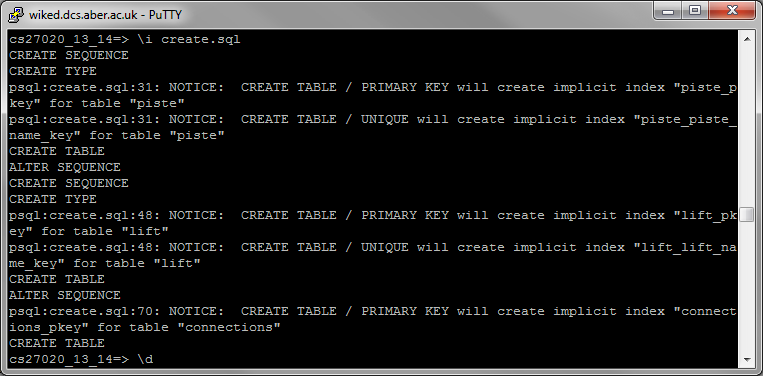
\includegraphics[width=1\textwidth]{IMG/create_tables.png}
 \caption{The output when creating tables.}
\end{figure}
\begin{figure}[H]
  \centering
    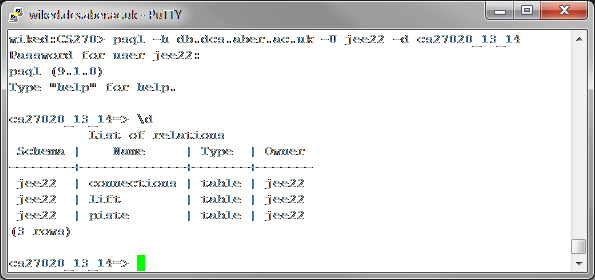
\includegraphics[width=1\textwidth]{IMG/completed_tables.png}
 \caption{The list of relations after running the create typescript.}
\end{figure}

\subsection{Data Types Justification}
Most data types have the contraint that they are 'NOT NULL'. When dealing with certain aspects of real data, such as a Piste or Lift, that definitely does have a specfic state (open/operating), specific numbers for lengths, rises and summits, and must have a name, I felt that NOT NULL should be included. There are no items in the sample data that have empty values for attributes.
\subsubsection{Piste}
\begin{itemize}
\item piste\_uid - int NOT NULL
The piste\_uid is kept as an integer to be a Unique Identification number. This way of using an integer allows it to be incremented for the number of values.
\item piste\_name - varchar(50) UNIQUE NOT NULL 
varchar allows the input of text, so the user can specify the name of the Lift. Setting the limit at 60 allows for a decent amount of characters without allowing unreasonable amounts. By using the constraint 'UNIQUE', it is enforcing the user to never have two of the same named Pistes.
\item grade - grade\_rank NOT NULL
I made a custom TYPE of ENUM for grade\_rank, allowing the user to select from the different types of ranks, and using an ENUM allows for future expansion on these grades if necessary.
\item length\_km - real NOT NULL
Using a real allows some floating point precision. Since the km is used to represent the length, where there can be numbers after the decimal, a real seemed appropriate to reprsent this data.
\item fall\_m - integer NOT NULL
A way to represent the fall as a whole number.
\item open\_piste - boolean
Since a piste can either be open or not open, a true/false boolean seemed appropriate to determine either/or.
\end{itemize}

\subsubsection{Lift}
\begin{itemize}
\item lift\_uid - int NOT NULL\\
The lift\_uid is kept as an integer to be a Unique Identification number. This way of using an integer allows it to be incremented for the number of values.
\item lift\_name - varchar(60) UNIQUE NOT NULL
varchar allows the input of text, so the user can specify the name of the Lift. Setting the limit at 60 allows for a decent amount of characters without allowing unreasonable amounts. By using the constraint 'UNIQUE', it is enforcing the user to never have two of the same named Lifts.
\item lift\_type - type\_lift NOT NULL
I made a custom TYPE of ENUM for lift\_type, allowing the user to select from the types of lift in the sample data, and using an ENUM allows for future expansion on types if necessary.
\item summit\_m - integer NOT NULL
A way to represent the summit as a whole number.
\item rise\_m - integer NOT NULL
A way to represent the rise as a whole number.
\item length\_m - integer NOT NULL
A way to represent the length as a whole number.
\item operating - boolean
Since a lift can either be operating or not operating, a true/false boolean seemed appropriate to determine either/or.
\end{itemize}

\subsection{Quering the Database}
\subsubsection{Test Data}
In order to test my data, I wrote the sample data into a typescript to insert it into my database. I will not include the typescript here. However, here are the contents of each relation after the insertion:


Where you might see \textless and \textgreater in the Test Query typescripts, it should be assumed that here is where a value would go for the query. An example would be '\textless lift\_name \textgreater ' could be imagined to be 'Rastlift', or any other lift\_name, when executing the query.
\subsubsection{Erronous Data Entry}
In order to check that my database was working correctly, I conducted a series of tests where I attempted to INSERT incorrect data. Doing this confirmed that my database was robust and built as intended. Below are a series of screenshots and captions detailing my testing.

\subsubsection{Test Query 1}
"Return the pistes served by a given lift."
\begin{lstlisting}
SELECT * 
FROM piste WHERE piste_uid IN 
	(SELECT piste_uid
		FROM connections WHERE lift_uid IN 
	(SELECT lift_uid
		FROM lift WHERE lift_name='<lift_name>'));
\end{lstlisting}
\subsubsection{Test Query 2}
"Return the lift(s) that provide access to a given piste."
\begin{lstlisting}
SELECT * 
FROM lift WHERE lift_uid IN 
	(SELECT lift_uid 
		FROM connections WHERE piste_uid IN 
	(SELECT piste_uid 
		FROM piste WHERE piste_name='<piste_name>'));
\end{lstlisting}
\subsubsection{Test Query 3}
"Return the lifts that are currently operating."
\begin{lstlisting}
SELECT lift_name, operating 
	FROM lift WHERE operating='t';
\end{lstlisting}
\subsubsection{Test Query 4}
"Return the pistes that are currently open, together with the lifts that are currently operating and that provide access to those pistes."
\begin{lstlisting}
SELECT * FROM connections WHERE lift_uid IN
	(SELECT lift_uid FROM lift WHERE operating='t')
AND piste_uid IN
	(SELECT piste_uid FROM piste WHERE open_piste='t');
\end{lstlisting}
\newpage

\begin{thebibliography}{9}

\bibitem{sample}
  Edel Sherratt,
  \emph{CS27020 Assignment: Ski Lifts and Pistes}.
  Computer Science Department,
  Aberystwyth University,
  2014.

\end{thebibliography}

\end{document}
